\section{Описание взаимодействия спаренных наночастиц в дипольном приближении}

В данном параграфе будет рассмотрено ближнепольное взаимодействие двух золотых наностержней в дипольном приближении и продемонстрировано явление смещения резонанса ЛПП при изменении расстояния между наностержнями.
При падении периодического электромагнитного излучения на наночастицу в ней наводится дипольный момент. Тогда взаимодействие двух наночастиц можно представить как взаимодействие двух точечных диполей. Теоретическое описание взаимодействия таких диполей приведено в статье \cite{dipoleInteraction}.

Пусть один из двух диполей находится в начале декартовой системы координат (диполь (1)), а второй диполь находится на расстоянии $ r $ от первого вдоль оси $ Oz $. Энергия взаимодействия возникает вследствие взаимной поляризации, которая вычисляется следующим образом.

Пусть мгновенная поляризация диполя (1) задается следующим выражением:
\begin{equation}
\textbf{P} (1, t) = \textbf{P} \exp (-\imath \omega t),
\label{eq:instdipole1}
\end{equation}
где $ \omega $ --- частота внешнего электромагнитного поля.
Тогда векторный потенциал $ \textbf{A} $ и скалярный потенциал $ \phi $ в произвольной точке на расстоянии $ r $ от диполя определяются формулами

\begin{equation}
\textbf{A}(r, t) = - \frac{\imath \omega}{c} \textbf{P} \exp (-\imath \omega t) \frac{\exp (\imath \omega r / c)}{r},
\label{eq:vectorpotential}
\end{equation}
и
\begin{equation}
\phi(r, t) = \frac{\textbf{P} \cdot \textbf{r}}{r^2} \left( \frac{1}{r} - \frac{\imath \omega}{c} \right) \exp (-\imath \omega t) \exp (\imath \omega r / c),
\label{eq:scalarpotential}
\end{equation}
где $ c $ --- скорость света в вакууме. Соответствующее электрическое поля задается выражением:
\begin{equation}
\textbf{E} (r, t) = - \frac{1}{c} \dfrac{\partial \textbf{A}}{\partial t} - \nabla \phi.
\label{eq:elecdipolefromvector}
\end{equation}
Следовательно, получим $ \textbf{E}(r, t) = \textbf{E} (r) \exp(- \imath \omega t) $, где:

\begin{equation}
\textbf{E} = \frac{\textbf{P}}{r} \left( \frac{\omega ^2}{c^2} + \frac{\imath \omega}{c r} - \frac{1}{r^2} \right) \exp(\imath \omega r/c) - (\textbf{P} \cdot \textbf{r}) \frac{\textbf{r}}{r^3} \left( \frac{\omega ^2}{c^2} + \frac{3 \imath \omega}{c r} - \frac{3}{r^2} \right) \exp(\imath \omega r/c).
\label{eq:elecdipole}
\end{equation}
Значит, если $ \vert \textbf{r} \vert $ --- расстояние между диполями, а $ \textbf{r} $ --- направление вдоль оси $ Oz $, то компоненты $ \textbf{E}(1) $, вызванные диполем (1) при положении диполя (2), выражаются следующими формулами:

\begin{equation}
E_x (1) = f(r) P_x (1), \quad
E_y (1) = f(r) P_y (1), \quad
E_z (1) = h(r) P_z (1),
\label{eq:fieldcertesian}
\end{equation}
где
\begin{equation}
f(r) = \frac{\exp (\imath \omega r /c)}{r} \left( \frac{\omega ^2}{c^2} + \frac{\imath \omega}{c r} - \frac{1}{r^2} \right), \quad
h(r) = \frac{2 \exp (\imath \omega r /c)}{r} \left( \frac{1}{r^2} - \frac{\imath \omega}{c r} \right).
\label{eq:hf_functions}
\end{equation}
Это поле поляризует диполь (2), поляризация которого равна:
\begin{equation}
\textbf{P}(2) = \widehat{\alpha}(2) \textbf{E}(1),
\label{eq:polar2to1}
\end{equation}
где $ \widehat{\alpha} (2) $ -- тензор поляризуемости второго диполя. Эта индуцированная поляризация в свою очередь создает электрическое поле в первом диполе, наводя свою поляризацию, и в соответствии с формулой (\ref{eq:polar2to1}) получим:
\begin{equation}
\textbf{P}(1) = \widehat{\alpha}(1) \textbf{E}(2).
\label{eq:polar1to2}
\end{equation}
Из формул (\ref{eq:fieldcertesian}), (\ref{eq:polar2to1}) и (\ref{eq:polar1to2}) получим:
\begin{equation}
\textbf{P}(2) = \widehat{X}(2) \textbf{P}(1), \quad 
\textbf{P}(1) = \widehat{X}(1) \textbf{P}(2),
\label{eq:polarity}
\end{equation}
где матрицы $ \widehat{X} $ определяются следующим образом:
\begin{equation}
\widehat{X} = \left(
\begin{matrix}
\alpha _{11} f & \alpha _{12} f & \alpha _{13} h \\
\alpha _{21} f & \alpha _{22} f & \alpha _{23} h \\
\alpha _{31} f & \alpha _{31} f & \alpha _{33} h \\
\end{matrix}
\right),
\label{eq:Xmatrix}
\end{equation}
и $ \alpha _{ij} $ являются матричными элементами тензоров поляризуемости $ \widehat{\alpha}(1) $ и $ \widehat{\alpha}(2) $, соответственно. Уравнения (\ref{eq:polarity}) обеспечивают условие согласования на разрешенные моды:
\begin{equation}
\textbf{P}(1) = \widehat{Y} \textbf{P}(1), \quad
\widehat{Y} = \widehat{X}(1) \widehat{X}(2).
\label{eq:allowedmodes}
\end{equation}
Частоты разрешенных мод задаются дисперсионным соотношением:
\begin{equation}
D(\omega) \equiv \det (\widehat{I} - \widehat{Y}) = 0.
\label{eq:dispersiondipole}
\end{equation}

Из уравнений (\ref{eq:Xmatrix}) и (\ref{eq:allowedmodes}) компоненты матрицы $ \widehat{Y} $ имеют вид:
\begin{subequations}
\begin{gather}
y_{11} = \{\alpha_{11}(1) \alpha_{11}(2) + \alpha_{12}(1) \alpha_{21}(2)  \} f^2 + \alpha_{13}(1) \alpha_{31}(2) fh , \label{eq:y11} \\
y_{22} = \{\alpha_{21}(1) \alpha_{12}(2) + \alpha_{22}(1) \alpha_{22}(2)  \} f^2 + \alpha_{23}(1) \alpha_{32}(2) fh , \label{eq:y22} \\
y_{33} = \{\alpha_{31}(1) \alpha_{13}(2) + \alpha_{32}(1) \alpha_{23}(2)  \} fh + \alpha_{33}(1) \alpha_{33}(2) h^2 , \label{eq:y33} \\
y_{12} = \{\alpha_{11}(1) \alpha_{12}(2) + \alpha_{12}(1) \alpha_{22}(2)  \} f^2 + \alpha_{13}(1) \alpha_{32}(2) fh , \label{eq:y12} \\
y_{13} = \{\alpha_{11}(1) \alpha_{13}(2) + \alpha_{12}(1) \alpha_{23}(2)  \} fh + \alpha_{13}(1) \alpha_{33}(2) h^2 , \label{eq:y13} \\
y_{23} = \{\alpha_{21}(1) \alpha_{13}(2) + \alpha_{22}(1) \alpha_{23}(2)  \} fh + \alpha_{23}(1) \alpha_{33}(2) h^2 . \label{eq:y23}
\end{gather}
\end{subequations}
Матричные элементы $ y_{21} $, $ y_{31} $ и $ y_{32} $ получаются из уравнений (\ref{eq:y12}), (\ref{eq:y13}) и (\ref{eq:y23}) путем перестановки индексов 1 и 2 диполей. Например, $ y_{21} = y_{12} \{ (1) \rightleftarrows (2) \} $. 

Возьмем модель двух взаимодействующих золотых эллипсоидов. Тогда тензор поляризуемости будет анизотропным. Пусть $ \alpha = \alpha_{xx} = \alpha_{11} \neq 0 $, а остальные компоненты равны нулю, что соответствует состоянию, в котором резонансная частота, возбужденная электрическим полем вдоль оси $ Ox $, находится вдали от других резонансных частот. Тогда матрица (\ref{eq:Xmatrix}) преобразуется в матрицу:
\begin{equation}
\widehat{X} = \left(
\begin{matrix}
\alpha f & 0 & 0 \\
0 & 0 & 0 \\
0 & 0 & 0 \\
\end{matrix}
\right).
\label{eq:Xmatrix_dipole}
\end{equation}

Используя уравнение (\ref{eq:polarizabilityEllip}) для поляризуемости эллипсоида и подставляя формулу Друде (\ref{eq:EpsilonFreeElectron}) для диэлектрической проницаемости металла, получим уравнение поляризуемости:
\begin{equation}
\alpha = \frac{\omega_p^2}{\omega_p^2 - \omega ^2 / L_x} \frac{V}{4 \pi},
\label{eq:polarizability_dipole}
\end{equation}
где $ \omega_p $ -- плазменная частота металла, $ L_x $ -- фактор деполяризации эллипсоида, определяемый формулой (\ref{eq:Lfactor}), $ V $ -- объем эллипсоида. Дисперсионное соотношение (\ref{eq:dispersiondipole}) преобразуется к виду:
\begin{equation}
\alpha f = \pm 1.
\label{eq:dispersion_dipole}
\end{equation}
Рассмотрим ближнепольный случай, для которого $ r \ll \lambda $. Тогда множитель $ \exp (\imath k r) $ функции $ f(r) $, где $ k = \omega / c $, можно разложить в ряд Тейлора. Тогда для функции $ f(r) $ получим уравнение:
\begin{equation}
f(r) = \frac{\exp (\imath k r)}{r} \left( k^2 + \frac{\imath k}{r} - \frac{1}{r^2} \right) \simeq \frac{1}{r} \left( 1 + \imath k r - \frac{k^2 r^2}{2} + ... \right) \left( k^2 + \frac{\imath k}{r} - \frac{1}{r^2} \right).
\label{eq:f_Taylor}
\end{equation}
Так как $ k r \ll 1 $, то $ \frac{1}{(kr)^2} \gg \frac{1}{kr} $ и $ \frac{1}{(kr)^3} \gg \frac{1}{kr} $ и пренебрегая членами порядка $ r^n $, где $ n \geq -1 $, получим:
\begin{equation}
f(r) \simeq \frac{1}{r^3}.
\label{eq:f_dipole}
\end{equation}
Подставляя (\ref{eq:f_dipole}) в (\ref{eq:dispersion_dipole}), получим уравнение для собственных частот:
\begin{equation}
\omega_{\pm} = \omega_p \sqrt{L_x} \sqrt{1 \mp \frac{V}{4 \pi r^3}}.
\label{eq:freq_dipole}
\end{equation}
Выражая уравнение (\ref{eq:freq_dipole}) в длинах волн, получим:
\begin{equation}
\lambda_{\pm} = \frac{\lambda_p}{\sqrt{L_x}} \frac{1}{\sqrt{1 \mp V / 4 \pi r^3}},
\label{eq:wl_dipole}
\end{equation}
где $ \lambda_p $ -- плазменная длина волны.

Рассмотрим два эллипсоида, у которых длины полуосей равны 75 нм вдоль оси $ Ox $,  15 нм вдоль оси $ Oy $ и 25 нм вдоль оси $ Oz $.  Для таких эллипсоидов фактор деполяризации вдоль оси $ Ox $ $ L_x \approx 0.08  $. Объем одного эллипсоида $ V \approx 1.18*10^5 $ нм$ ^3 $. Взаимное расположение этих 
эллипсоидов показано на рис.~\ref{img:semianalytical_dd}a. Значение плазменной частоты $ f_p = \omega_p / 2 \pi $ взято из статьи \cite{plasma_freq} и составляет $ 2.183*10^{15} $ Гц.

\begin{figure}[h]
\center{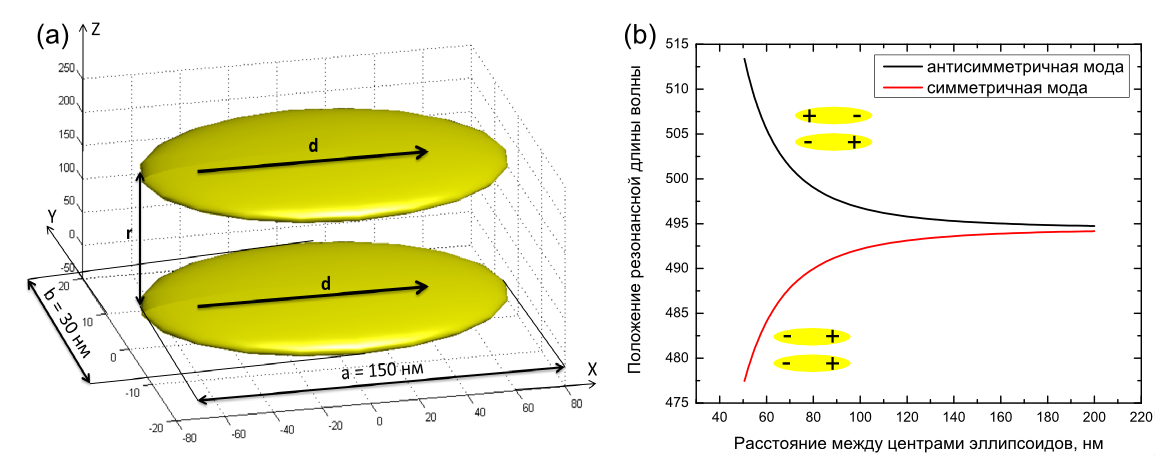
\includegraphics[width=16cm]{img/fenomenology.png}}
\caption{Взаимное расположение двух эллипсоидов из золота и направление дипольного момента $ \textbf{d} $ (а), зависимость резонансной длины волны от расстояния $ r $ между центрами эллипсоидов (b).}
\label{img:semianalytical_dd}
\end{figure}

Зависимость резонансной длины волны от расстояния между центрами эллипсоидов показано на рис.~\ref{img:semianalytical_dd}b. На больших расстояниях взаимодействия между частицами нет, поэтому каждую частицу можно предположить одиночной, с собственной резонансной длиной волны $ \lambda_{isolated} \approx  495 $ нм. При взаимодействии двух частиц появляется расщепление на две моды: симметричную с большей энергией взаимодействия и антисимметричную с меньшей энергией взаимодействия. При расстояниях $ r \ll \lambda $ в однородных внешних полях антисимметричная мода возбуждается неэффективно, поэтому больший интерес представляет симметричная мода, на которой построены принципы <<плазмонной  линейки>>. Мгновенное распределение зарядов в симметричном  и антисимметричном случае показано на рис.~\ref{img:semianalytical_dd}b. 